\chapter{Systeemarchitectuur}
\label{chap:architectuur}

\section{Model}
\label{sec:model}
CalZone is een webapplicatie. Gebruikers van het systeem bezoeken de applicatie via hun webbrowser. 
Deze browser kan de browser op hun computer zijn of de webbrowser op hun smartphone.
Doorheen de ontwikkeling van het project wordt de focus vooral gericht op Android toestellen en browsers op deze toestellen wat betreft het mobiele aspect van de applicatie.
\\
CalZone heeft als architectuur gekozen voor het MVC-patroon.\cite{mvc}

\begin{figure}[H]
	\centering
	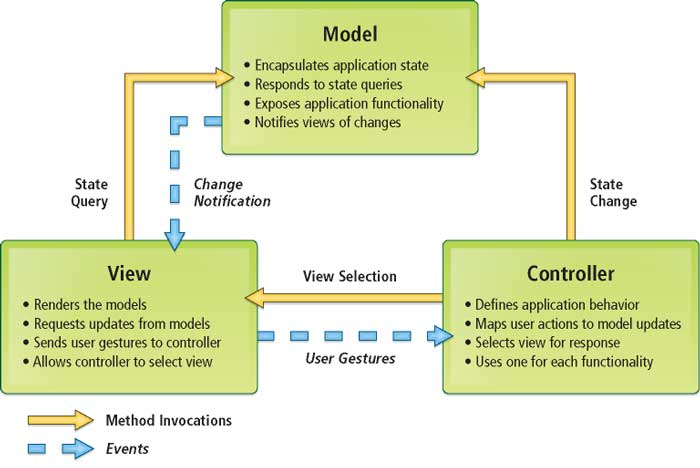
\includegraphics[scale=0.5]{img/mvc}
	\label{fig:mvc}
	\caption{Een voorstelling van de werking van een systeem gebruikmakende van een MVC architectuur}
\end{figure}

\section{Gebruikte technologie}
\label{sec:technologie}
De programmeertaal die gebruikt wordt, is Java. 
In Java wordt gebruik gemaakt van het Spring MVC framework\cite{spring, spring-mvc} voor het ontwikkelen van CalZone. 
De IDE waarin geprogrammeerd wordt, is de meest recente versie van 'Eclipse Classic' met volgende uitbreidingen:

\begin{itemize}
	\item De gehele collectie 'Web, XML, Java EE and OSGi Enterprise Development'	
	\item Spring Tool Suite (uit de Eclipse Marketplace)
	\item De gehele collectie 'Maven Integration for Eclipse'
\end{itemize}
\noindent
Het uitvoeren van de applicatie wordt mogelijk gemaakt door middel van Apache Maven\cite{Maven} en Apache Tomcat\cite{Tomcat}.
De gebruikte databank voor de back-end is MySQL.
De connecties vanuit het logisch niveau van het systeem naar de databank verlopen via Hibernate\cite{hibernate}. 
Voor de view wordt gebruik gemaakt van JSP's: een technologie om dynamisch webpagina's te genereren.\\

De applicatie moet in staat zijn om lessenroosters te maken.
Om dit doel te verwezenlijken wordt gebruik gemaakt van OptaPlanner \cite{optaplanner}. 
Meer uitleg over OptaPlanner en het maken van lessenroosters staat beschreven in \ref{subsec:scheduler}, \ref{subsec:scheduleclass} en \ref{subsec:scheduling}.